% ===========================================================================
% Dual-Rate Routed Attention for Efficient Long-Horizon Time-Series
% Forecasting -- workshop draft (NeurIPS-style layout)
%
% How to compile: pdflatex -> bibtex -> pdflatex -> pdflatex (or use the
% Overleaf "NeurIPS 2026" template and paste the files in). See README.md.
%
% NOTE ON THE STYLE FILE: paper/neurips_2026.sty is a self-contained layout
% fallback. Replace it with the official NeurIPS style before submission;
% the rest of this preamble is written to match the official template.
% ===========================================================================
\documentclass{article}

\usepackage[preprint]{neurips_2026}

\usepackage[utf8]{inputenc}
\usepackage[T1]{fontenc}
\usepackage{graphicx}
\usepackage{booktabs}
\usepackage{amsfonts}
\usepackage{microtype}
\usepackage{xcolor}
\usepackage{url}
\usepackage{hyperref}

% relax overly-tight paragraph breaking in the working draft
\emergencystretch=1.5em

% --- working-draft markers (remove all TODO/NEEDS-VERIFICATION before
%     submission; grep for "TODO:" and "NEEDS VERIFICATION" to find them) ---
\newcommand{\todo}[1]{\textbf{\textcolor{red!70!black}{[TODO: #1]}}}
\newcommand{\needverify}[1]{\textbf{\textcolor{orange!90!black}{[NEEDS VERIFICATION: #1]}}}

% --- title and authors -----------------------------------------------------
% TODO: fill in real authors/affiliations before submission.
\title{Dual-Rate Routed Attention for Efficient Long-Horizon Time-Series Forecasting}

\author{%
  Author Name$^1$ \\ \texttt{email@example.com}
  \And
  Second Author$^2$ \\ \texttt{email2@example.com} \\
  $^1$Affiliation 1 \quad $^2$Affiliation 2
}

\begin{document}

\maketitle

\begin{abstract}
Long-horizon time-series forecasting with Transformers is dominated by the
cost of quadratic attention over long lookback windows. Compressed-and-indexed
attention---compressing the key/value (KV) stream and routing each query to a
few compressed blocks---reduces this cost, but its design space is rarely
studied systematically. We treat the family as a two-axis design problem: the
KV compression rate $c_{KV}$ and the routing resolution $c_R$. Under a frozen
direct-96-step forecasting protocol with twenty-five paired seeds, we run a
parameter-equalized $2\times2$ factorial on ETTh1 and a three-way
comparison---full attention, the equal-rate CSA configuration $(4,4)$ (the
design point of DeepSeek-V4's Compressed Sparse Attention), and the dual-rate
corner DRRA $(8,4)$---across twelve datasets spanning the ETT family, large
multivariate series, different dynamics, and mechanistic synthetic probes. We
report four findings. First, on ETTh1 \emph{every} compressed configuration
outperforms full causal attention on validation MSE (mean deltas $-16.6\%$
to $-26.2\%$, in 96/100 paired seed comparisons; Holm-adjusted
$p \approx 7\times10^{-5}$) at an equal or slightly smaller parameter
count; a bit-exact wiring audit confirms the baseline is correctly
implemented. Second, coarsening the router ($c_R{:}4{:}1 \to 8{:}1$)
systematically deteriorates accuracy ($+0.029$ validation MSE), while
coarsening KV compression is mildly beneficial ($-0.052$): the pre-registered
decoupling hypothesis is supported on ETTh1 (per-seed paired contrast, exact Wilcoxon $p = 0.0023$)---
routing granularity carries accuracy there, while KV content density is mildly beneficial.
Third, the best-mean ETTh1 cell DRRA $(8,4)$ reduces the attention matrix to 48 (+1 sink)
columns
versus 256 (5.22$\times$) at a matching parameter count. Fourth, the advantage
is \emph{signal-dependent}: 8/12 datasets (DRRA) and 7/12 (CSA), concentrated
on smooth, redundant real-world series, with slight losses on the synthetic
exact-recall probes. The factorial conclusions are statistically established
at $n{=}25$; the cross-dataset pattern remains descriptive (five seeds per
dataset, per-dataset tests capped at $p = 0.0625$), and latency is reported
for the development machine only.
\end{abstract}

\section{Introduction}
\label{sec:intro}

Long-horizon time-series forecasting---predicting the next $H$ steps from a
lookback window of length $L$---is a core task in energy, traffic, and
finance applications. Transformer-based forecasting models \citep{zhou2021informer,nie2023patchtst,liu2024itransformer}
are accurate but pay a quadratic cost $O(L^2)$ in the attention mechanism as
the lookback grows. One widely used remedy is \emph{compressed-and-indexed}
attention: compress the $L$ key/value (KV) positions into $C = L / c_{KV}$
blocks, and have each query attend to only a small, \emph{routed} subset of
those blocks plus a local sliding window. This family underlies recent
efficient-attention designs for large language models
\citep{yuan2025nsa,deepseekv4_2026}, and its components---content-based
routing \citep{roy2020routing}, low-rank KV compression
\citep{deepseekv2_2024}---are individually well known.

What is not well studied is the \emph{design space} of this family: how the
two independent compression axes interact. We identify two axes:
\begin{itemize}
  \item \textbf{KV compression rate} $c_{KV}$: how aggressively the content
        stream is compressed into blocks ($C = L / c_{KV}$ blocks);
  \item \textbf{Routing resolution} $c_R$: how finely the router represents
        the history when deciding which blocks to attend to
        ($M = L / c_R$ index tokens).
\end{itemize}
Coarsening either axis cuts compute, but the two axes may not trade
accuracy equally. Our central question is therefore a controlled, empirical
one: \emph{which axis carries accuracy, and which axis only buys
efficiency?}

This paper is a \textbf{design study}, not a proposal of a new attention
mechanism: every building block we use is a configuration of known ideas
(Section~\ref{sec:method}), and overlaps with concurrent work
\citep{yuan2025nsa,deepseekv4_2026} are acknowledged rather than elided
(Section~\ref{sec:related}). Our contributions are:
\begin{enumerate}
  \item[(a)] \textbf{A controlled $2\times2$ factorial design.} All four
        combinations of $c_{KV}, c_R \in \{4{:}1, 8{:}1\}$ are evaluated on a
        frozen task---ETTh1, direct 96-step forecasting---under an
        \emph{auxiliary-identical} contract (identical window, top-$k$, heads,
        hidden size, optimizer, schedule) with attention-parameter
        equalization to within $0.3\%$, across five paired seeds
        (Section~\ref{sec:experiments}).
  \item[(b)] \textbf{A decoupled-rate finding (directional).} Coarsening the
        router deteriorates accuracy ($+0.046$ validation MSE for
        $c_R{:}4{:}1 \to 8{:}1$), while coarsening KV compression is
        mildly beneficial ($-0.043$). The best cell $(c_{KV}{=}8, c_R{=}4)$
        reduces the attention matrix 5.3$\times$ relative to full attention
        at equal parameters. We report these as directional observations:
        effect sizes are smaller than the within-cell seed standard
        deviation, and no significance test has been run.
  \item[(c)] \textbf{An honest efficiency/accuracy characterization.} A
        surprising---and wiring-verified---baseline result: all compressed
        configurations beat full causal attention on the frozen task
        ($-18.5\%$ to $-29.1\%$ validation MSE), with explicit limitations
        (single dataset, CPU-scale models, descriptive statistics).
  \item[(d)] \textbf{Reproducibility artifacts.} A frozen task specification,
        machine-readable results manifests, a verified parameter registry,
        causality-verification suites, and a codebase in which every reported
        number traces to a file (Appendix~\ref{sec:appendix-repro}).
\end{enumerate}

\textbf{Scope and non-claims.} This work does not claim a novel attention
mechanism, does not claim state-of-the-art forecasting accuracy (no external
baselines are run yet), does not claim statistical equivalence or
significance (descriptive statistics only, five seeds), and does not report
wall-clock speedups: the pre-freeze latency figures from earlier stages of
this project are superseded and are deliberately \emph{not} used here.
Measured latency, FLOPs, and hardware transfer are
planned follow-up work (Section~\ref{sec:discussion}).

\section{Related Work}
\label{sec:related}

\subsection{Routed and compressed attention}
The general idea of content-based routing goes back to the Routing
Transformer \citep{roy2020routing}, which clusters tokens with online
$k$-means and restricts attention to tokens in the same cluster. Native
Sparse Attention (NSA) \citep{yuan2025nsa} combines coarse-grained token
compression with fine-grained token selection, making it the closest
conceptual cousin of the family studied here. DeepSeek-V4's hybrid
attention \citep{deepseekv4_2026} pairs a Compressed Sparse Attention (CSA)
stage with a Heavily Compressed Attention (HCA) stage for million-token
contexts, reporting $27\%$ of single-token inference FLOPs and $10\%$ of KV
cache versus DeepSeek-V3.2; we adopt the working name ``Dual-Rate Routed
Attention'' (DRRA) for our family in part to avoid colliding with that
label, and refer to the equal-rate configuration point that matches
CSA's rate settings as ``CSA'', following DeepSeek's terminology
(Section~\ref{sec:method}).
The low-rank KV bottleneck and shared-query projection used in our
configurations descend from Multi-head Latent Attention (MLA)
\citep{deepseekv2_2024}. Attention distillation toward cheaper inference
architectures \citep{goldstein2025radlads} overlaps a secondary, separable
thread of this project (Appendix~\ref{sec:appendix-surrogate}) rather than
the routing/compression core studied here.

Crucially for our claim (b), none of these works, to our knowledge,
\emph{systematically varies the content-compression rate and the routing
resolution independently and reports their separate main effects} on a
fixed task. The closest are Simplified Sparse Attention
\citep{mao2026ssa}, which compresses context into gist tokens and
selectively unfolds top-$k$ chunks but derives $k$ from the chunk size to
hold the total budget constant (Eq.~A.1), coupling the two axes; and The
Sparse Frontier \citep{nawrot2025sparsefrontier}, which sweeps selection
budgets across six methods with no content-compression knob.
DeepSeek-V4 \citep{deepseekv4_2026} and NSA \citep{yuan2025nsa} expose
both mechanisms as fixed hyperparameters without varying them
independently. Two structural differences are worth naming. First,
terminology: DeepSeek-V4 has no ``router'' --- its \emph{Lightning Indexer}
scores compressed KV entries and a \emph{top-$k$ selector} subsamples them
(Section~\ref{sec:family-mech} adopts the generic term ``router'' for this
scorer-plus-selector pair). Second, in CSA the indexer's key stream is
compressed with the \emph{same} operation and rate $m$ as the KV entries,
so the scoring granularity is tied to the KV compression rate; in our
family the indexer stream has its own rate $c_R$, which is precisely the
axis the factorial varies. We confirmed this on a systematic sweep of the 2024--2026
routing/compression-attention literature (August 2026).

Mixture-of-block attention (MoBA) \citep{lu2025moba} is the closest
selection-only relative: it partitions the raw KV cache into blocks and
routes each query to the top-$k$ blocks through a gating function, so block
size sets the selection granularity and $k$ the realized budget. The
contrast sharpens both axes of our design. First, MoBA's content stream is
the uncompressed cache --- the only granularity knob is the block size, and
it is the same knob as the selection unit; our family instead compresses
the content stream at rate $c_{KV}$ (KV-cache compression) and scores a
separately compressed index stream at rate $c_R$ (routing resolution),
which is what lets the two axes vary independently. Second, holding the
top-$k$ count fixed while $c_R$ changes --- our operating protocol ---
changes how many valid blocks each query actually reads, whereas MoBA
reports block size and $k$ jointly and discusses holding the attended
budget roughly constant across granularities; the realized-coverage
caveat in Section~\ref{sec:rq2} states the consequence for our fixed-$k$
comparison, with a budget-matched control deferred rather than assumed
away (Appendix~\ref{sec:appendix-roadmap}). Third, MoBA trains
its selection pathway end to end, so its query and key streams adapt to
the routing they induce, while our indexer is parameter-free and receives
no task gradient (Section~\ref{sec:rq2} measures what that implies for
route stability in practice).

\subsection{Efficient and accurate time-series forecasting}
Long-horizon forecasting architectures include the ProbSparse-attention
Informer \citep{zhou2021informer}, patching-based PatchTST
\citep{nie2023patchtst}, the inverted iTransformer \citep{liu2024itransformer},
linear baselines \citep{zeng2023dlinear}, and 2D-variation modeling with
TimesNet \citep{wu2023timesnet}. Two of them, DLinear
\citep{zeng2023dlinear} and PatchTST \citep{nie2023patchtst}, have been run
under our frozen protocol as external reference points (not peer methods;
Section~\ref{sec:refpoints}); the rest are itemized as pending work in the
appendix future-work list, Appendix~\ref{sec:appendix-roadmap}. Our contribution is orthogonal: we do
not propose a new forecasting architecture but study two design axes of the
attention module that any of these models could use.

\subsection{Positioning summary}
This paper sits in the intersection of efficient attention and
time-series forecasting, as a \emph{controlled design study}: it measures
how two configurable axes of a fixed attention family trade off accuracy
and efficiency on one frozen task, and it does so with the reproducibility
discipline (pre-registered factorial, paired seeds, parameter
equalization, frozen task spec) that makes the trade-off structure
measurable rather than anecdotal.

\section{Method}
\label{sec:method}

\subsection{Task and evaluation protocol (frozen)}
\label{sec:task}
All experiments use a single frozen task specification---stated in full in
this section and frozen before any model-comparison run---applied to twelve
datasets: the Electricity Transformer Temperature (ETT) family
\citep{zhou2021informer} (ETTh1, ETTh2, ETTm1, ETTm2---7 features each, at
hourly ($h$) and 15-minute ($m$) sampling), the large multivariate sets Electricity (321
channels), Traffic (862), and Weather (21) and the Exchange rates (8,
daily), as benchmarked by \citet{wu2021autoformer} and redistributed by the
Time-Series Library \citep{wu2023timesnet}, Solar-Energy (137, 10-minute)
\citep{lai2018lstnet}, and three mechanistic synthetic families (controlled
sinusoids,
change points, and a delayed-copy task; 7 channels each) generated
deterministically from fixed seeds (Appendix~\ref{sec:appendix-roadmap}).
Each dataset is split chronologically $60\%/20\%/20\%$ into
train/validation/test with stride-1 sliding windows of length $L{=}256$ that
never span a split boundary. Normalization is a per-feature z-score whose
statistics are fit on the \emph{train} split only and applied to all splits
(the earlier practice of fitting over the full series was a future-statistics
leak and is fixed); channels with zero training variance are normalized with
unit scale. The task is \emph{direct} 96-step forecasting: in one forward
pass the model maps an input window $x \in \mathbb{R}^{B \times L \times F}$
to a forecast $\hat{y} \in \mathbb{R}^{B \times H \times F}$, where $B$ is the
number of windows in the batch, $L{=}256$ the lookback, $H{=}96$ the horizon,
and $F$ the number of features (channels) of the dataset. The loss is the
pooled mean squared error (MSE) over all $(B, H, F)$ elements, reported in
standardized units (lower is better).
No autoregressive decoding and no teacher forcing is used. Causality is
enforced by construction and verified empirically: a future-invariance and
exact-zero-future-gradient suite passes for every variant. Windows overlap
by 255/256 positions and are therefore not independent samples; this is a
declared limitation (Section~\ref{sec:limitations}).

Training is identical for every configuration: AdamW ($\mathrm{lr}{=}10^{-4}$,
weight decay $10^{-5}$), gradient clipping at norm 10, batch size 32, a
fixed budget of 10 epochs, float32 on CPU (Apple Silicon, 8 threads), and
deterministic seeding with the same seed used for data loading and model
initialization. The factorial is run at $n{=}25$ paired seeds: the five
pre-registered seeds $\{42, 123, 2024, 7, 99\}$ and a 20-seed power
extension (seeds 1--21 excluding the pre-registered set) run under the
byte-identical protocol and merged post hoc (Section~\ref{sec:rq1}). The
fixed 10-epoch budget is justified by learning-curve
analysis on the pre-registered-seed runs: all cells are in a plateau regime
after epoch 4 and the mean last-3-epoch drift across those 20 runs is
$+0.0009$; no cell keeps improving
systematically, so the budget does not bias cell comparisons.

\subsection{Model family}
\label{sec:family}
All configurations share one minimal Transformer block (hidden size
$d{=}128$, $h{=}4$ heads, head dimension $d_h{=}32$, hence
$d = h\,d_h$) with a horizon head
$\mathrm{Linear}(128 \rightarrow H \cdot F)$ applied to the last position:
\begin{equation}
e = \mathrm{input\_proj}(x) + \mathrm{pos\_embedding}, \qquad
z = \mathrm{MLP}(\mathrm{LN}(\mathrm{attn}(e) + e)), \qquad
\hat{y} = \mathrm{horizon\_head}(z[:, -1, :]),
\end{equation}
where $x$ is the input window of Section~\ref{sec:task}, $e$ the embedded
sequence, $\mathrm{LN}$ layer normalization, $\mathrm{MLP}$ the
feed-forward block, and $z$ the block output; $z[:, -1, :]$ is its last
position, the only position the forecast head reads. The only difference
between configurations is the attention module. The shared Q/KV/O
(query, key--value, output) projections follow the MLA-style pattern: a
low-rank query projection with root-mean-square normalization (RMSNorm), a
tied single-head KV projection ($K = V$) with rotary position embeddings
(RoPE) applied to the last 8 of the $d_h{=}32$ dimensions, and a grouped
output projection.
A full causal attention variant (\emph{Normal}) with no compression serves
as the task-appropriate baseline.

Figure~\ref{fig:arch} draws the two paths side by side at the same level of
detail, so that the quantity that separates the two families---how many key
columns a query reads---can be read from the figure rather than inferred from
the prose. Panel~(a) reads all $L$
columns under a causal mask. Panel~(b) reads a column set assembled from
three sources---$L/c_{KV}$ compressed blocks, the last $W{=}16$ positions
kept at full resolution, and one learned sink---and each attention box
carries a strip marking those columns. Two properties of panel~(b) carry
into the rest of the paper. Its per-query column count grows as $L/c_{KV}$
plus a constant (the window and the sink), rather than as $L$, so at fixed
rates the saving is a constant factor and not a change of asymptotic order;
Section~\ref{sec:forecast} therefore reports it as a ratio that saturates
rather than as a speedup that compounds with context. And the selection is
applied as a mask rather than as a reduction in work---every block column is
computed either way---so the arithmetic is set by the two rates and not by
which blocks are kept, and what the selection does buy is measured in
Section~\ref{sec:controls}.

\begin{figure}[t]
\centering
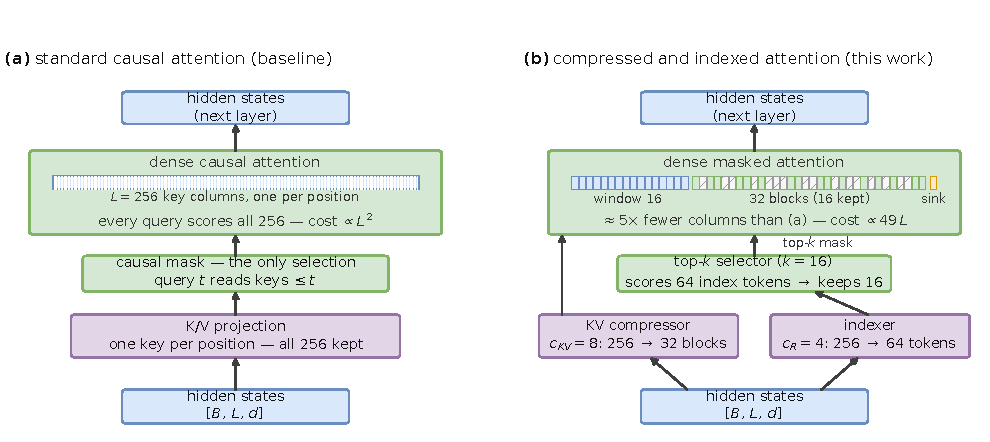
\includegraphics[width=\linewidth]{figures/fig1_architecture_compare.pdf}
\caption{The attention module, standard beside compressed. Both panels start
from the same hidden-state tensor $[B, L, d]$ ($B$ = batch size, $L$ =
lookback, $d$ = hidden size) and feed the next layer. \textbf{(a)}~Standard
causal attention, the \emph{Normal} baseline: every position keeps its own key
and value, so each query scores all $L{=}256$ keys, restricted only by the
causal mask---cost growing with $L^2$. \textbf{(b)}~The compressed-and-indexed
module, drawn at the $(c_{KV}, c_R) = (8,4)$ cell ($c_{KV}$ = KV-cache
compression rate, positions per stored block; $c_R$ = routing resolution,
positions per index token). From the same hidden states, two branches run in
parallel: a KV compressor ($c_{KV}{=}8$: 256 positions $\to$ 32 blocks) and a
routing indexer ($c_R{=}4$: 256 positions $\to$ 64 index tokens). The router
scores the index tokens with the query and keeps the top-$k{=}16$; two index
tokens map to one block at this cell, so up to 16 of the 32 block columns are
attended. The 32 block columns, the sliding window (16 uncompressed
positions) and an always-visible sink column are combined into a fixed column
set of $16 + 32 + 1 = 49$, and attention is computed densely over that set
with unselected blocks masked to $-\infty$ (Section~\ref{sec:family-mech});
the hatched cells are the ones computed and then masked. Cost therefore
scales with the strip's width, 49 against 256, not with the selection. Both panels
share the Transformer block and the Q/KV/O projections; only the attention
module differs, and the horizon head maps the last hidden state to the
96-step forecast.}
\label{fig:arch}
\end{figure}

\subsection{The compressed-and-indexed attention family}
\label{sec:family-mech}
Each compressed configuration (Figure~\ref{fig:arch}) consists of three
components, all inherited verbatim from the reference implementation:

\textbf{Two-series compressor.} The $L$ positions are projected to double
width and gated by a per-dimension softmax over $2m$ slots, so that every
token contributes to two adjacent windows (its own and the next); the
weighted sum is RMSNormed and RoPE-encoded at block starts. With rate
$m$---the cell's KV compression rate, $m = c_{KV}$---this yields
$C = L/m$ KV blocks, block $j$ covering $[mj, mj + m - 1]$. The
same compressor, with its own parameters, produces the $M = L / m_{idx}$
routing index tokens, where $m_{idx} = c_R$ is the routing resolution. The
two rates are the only quantities the factorial varies
(Section~\ref{sec:factorial}); $C$ and $M$ are the column counts they imply.

\textbf{Router (scorer + top-$k$ selector).} Each query vector $q$ (one per
head, of dimension $d_h$) scores all $M$ index tokens as
$\mathrm{ReLU}(q \cdot \mathrm{idx}^\top)/\sqrt{d_h}$, where
$\mathrm{idx}$ denotes the index-token matrix and
$\mathrm{ReLU}(z) = \max(z, 0)$; the per-head scores are combined by a
head-mixing weight that is fixed in practice (see the trainability note
below). The router masks tokens that lie in the future and selects the
top-$k$ ($k{=}16$) of the remaining ones. We use ``router'' for the scorer-plus-selector
combination; DeepSeek-V4 \citep{deepseekv4_2026} calls the analogous scorer
the \emph{Lightning Indexer} and the selection step the \emph{top-$k$
selector} (their paper uses neither ``router'' nor a standalone indexer
module feeding the selector --- the indexer scores the KV entries, which the
selector then subsamples). In all compressed configurations the router reuses the
main query (shared-Q), valid because the query head dimension equals the
index head dimension; this removes one projection and one RoPE application.
The hard top-$k$ selection is non-differentiable, so the indexer parameters
(including CSA's dedicated $\mathrm{idx\_q\_proj}$) receive zero task-loss
gradient: no learning signal reaches the selector, and ``routing granularity'' effects in
this paper are selection-architecture effects, not learned routing. The released audit
logs both a zero gradient norm and a zero optimizer update delta for every
indexer-exclusive parameter, so those parameters are tracked by the optimizer rather
than absent from the graph. The audit
establishes gradient isolation, not literal route constancy---index scores are
computed from features produced by trainable upstream components, so the selected
set can change as those features drift over training. A route-overlap probe across
epochs measures that drift rather than assuming it away (Section~\ref{sec:probes});
a trained selector remains deferred future work (both audit limits are in the
released logs).

\textbf{Dense masked attention over the sparse selection.} Instead of
gathering the selected blocks, attention is computed densely over a fixed
column set---the $C$ KV blocks plus a sliding window of $W{=}16$---with
$-\infty$ masking of unselected blocks and a single learnable ``sink''
softmax column for stability. Masking to $-\infty$ makes the dense result
exactly equal to the sparse top-$k$ selection, with no approximation. On
CPU this formulation is several times faster than per-query gather in our
implementation, and it keeps the softmax exact.

\textbf{Index-to-block mapping (per cell).} The router selects top-$k{=}16$ index
tokens; index token $t$ covers $[4t, 4t{+}3]$ at $c_R{=}4$ ($[8t, 8t{+}7]$ at $c_R{=}8$)
and must be translated to KV-block id $j$ before the dense masked attention
($\sslash$ below denotes integer division):
\begin{itemize}
  \item $(8,4)$: two fine tokens per coarse block --- block $j = t \sslash 2$,
        covering $[8j, 8j{+}7]$ (at most two of the 16 selections collide per block).
  \item Equal-rate cells $(4,4)$, $(8,8)$: token $t$ \emph{is} block $t$ (identity).
  \item $(4,8)$: one coarse token fans out to two fine blocks $(2t, 2t{+}1)$,
        doubling the per-query selection to 32 block slots.
  \item Deeper ratios ($(16,4)$, $(32,4)$): $p$ fine tokens per coarse block --- block
        $j = t \sslash p$ with $p = 4, 8$ (the general many-to-one rule).
\end{itemize}
A selected block is read only when its entire span ends at or before the query
($\mathrm{block\_end} \le$ the query's position); otherwise --- and for tokens masked as future or
out of range --- it maps to a sentinel id that \_attend drops, so no query reads
future positions. Causality holds through the overlapping compressor as well: each
compressed block mixes only its own and the previous window (receptive field
$[m(j{-}1), mj{+}m{-}1]$), i.e.\ strictly backward, so the block-end guard is
sufficient. Any other $(c_{KV}, c_R)$ geometry raises instead of guessing a mapping
(the general rule above covers every tested cell).
The per-cell rule is exercised by a regression test at every tested rate pair and
at non-divisible token counts (Appendix~\ref{sec:appendix-repro}); an earlier
implementation applied the $(8,4)$ rule to every geometry, which is why the three
affected cells reported in Section~\ref{sec:experiments} are re-runs.

\subsection{The two design axes and the factorial}
\label{sec:factorial}
The two axes are the KV compression rate $c_{KV} = m$ and the routing
resolution $c_R = m_{idx}$. We evaluate the $2 \times 2$ factorial over
$c_{KV}, c_R \in \{4{:}1, 8{:}1\}$, i.e.\ cells $(4,4)$, $(8,4)$, $(4,8)$,
$(8,8)$. The two corners that also appear in the cross-dataset study are
referred to by name throughout:
\begin{itemize}
  \item \textbf{CSA} --- the equal-rate corner $(4,4)$, in which both axes
        sit at $4{:}1$. We adopt the \emph{name} of DeepSeek-V4's Compressed
        Sparse Attention \citep{deepseekv4_2026}, whose rate design point
        this cell matches: KV compression at rate $m{=}4$ (the same value used
        in DeepSeek-V4-Flash/Pro), routing/selection over entries at the
        same $4{:}1$ granularity, and a local sliding-window branch. The
        name marks the configuration, not an equivalence claim: we evaluate
        our own implementation at $L{=}256$ scale (selection budget
        $k{=}16$, window 16, versus their $k{\in}\{512, 1024\}$, window
        128), not DeepSeek-V4's mechanism (Section~\ref{sec:related}).
  \item \textbf{DRRA (Dual-Rate Routed Attention)} --- the dual-rate corner
        $(8,4)$ (coarse content, fine routing), which gives the family its
        working name. We use ``champion'' for this cell strictly as shorthand for
        ``the dual-rate corner'' (its efficiency geometry, not accuracy rank: on validation
        no cell is best, DRRA-vs.-CSA exact Wilcoxon $p = 0.62$); everywhere else we name
        the cell explicitly.
\end{itemize}
The remaining corners $(4,8)$ and $(8,8)$ appear only in the factorial.

\textbf{Why only $\{4,8\}^2$?} The grid is the pre-registered design (frozen
before any run), and a $2\times2$ factorial is the minimal design that
identifies both main effects and their interaction --- exactly the three
fixed effects of the deferred mixed-effects model. Grid extension was a
deliberate exclusion, for three reasons. First, the natural next points are
degenerate rather than informative: at $c_R{=}16$ the indexer stream has
only $L/16 = 16$ tokens, so the top-$k{=}16$ router selects \emph{all} of
them and routing collapses to attend-to-everything --- a $(\cdot,16)$ cell
would measure the no-routing endpoint, not finer routing (measuring the
latter would require raising $k$ as well, breaking the auxiliary-identical
contract that pairs all cells). Symmetrically, at $c_{KV}{=}16$ the KV
blocks ($16$) no longer outnumber the sliding window ($16$), so the column
composition changes what is being measured. Second, the two levels bracket
a $2\times$ range around the operating region of interest (the CSA corner
$(4,4)$ matches DeepSeek-V4's $m{=}4$), and both effect signs are
established within the bracket. Behavior outside the bracket was extrapolation
at pre-registration time; two deeper ratios, $(16,4)$ and $(32,4)$, were run later as
exploratory probes (same protocol) and are reported separately from the confirmatory
factorial (Section~\ref{sec:rq1}, Appendix~\ref{sec:appendix-exploratory}). The grid remains valid as the confirmatory design: the probes stay exploratory and never enter the confirmatory contrasts. Third, budget: each additional cell costs 25
paired runs ($\approx 6$ h CPU at the measured per-run cost of the seed
extension), and the $2\times2$ spends that budget on replication ---
statistical power for the pre-registered contrasts --- rather than on extra
cells. Adding off-grid cells (e.g.\ the $(\cdot,16)$ endpoint ablation,
roughly 1--2 h for 5 paired seeds) is straightforward in the harness and is
itemized as future work.
Table~\ref{tab:configs} lists the resulting geometry and
parameter counts.

\begin{table}[t]
\centering
\small
\caption{Configuration geometry and parameters (measured; attention module
and full model). All compressed cells share the auxiliary contract
(window 16 = tokens visible to every query, top-$k$ 16 = best-scoring index
tokens routed per query, 4 heads, head dimension 32, hidden 128, shared-Q
= one query projection shared by router and attention,
query/output projection ranks 64 = low-rank bottleneck dimensions) and differ only in
$(c_{KV}, c_R)$ = (KV-cache compression rate, routing resolution, in
positions per stored block and per index token); the low-rank
bottlenecks are equalized to within $0.27\%$ of the $(8,4)$ reference;
results for all cells are in Table~\ref{tab:factorial}. Starred rows are post-hoc exploratory probes, excluded from
all confirmatory contrasts. Columns: $C$ = KV blocks, $M$ = index tokens,
\emph{softmax cols} $= C + W + 1$ = KV blocks $+$ 16-token window $+$
always-visible sink column. Normal
attends to all 256 columns with no sink.}
\label{tab:configs}
\begin{tabular}{lcccccc}
\toprule
Config & $c_{KV}$ & $c_R$ & KV blocks $C$ & Index tokens $M$ & Softmax cols & Params (attn / full) \\
\midrule
Normal & --- & --- & --- & --- & 256 & 102{,}496 / 355{,}200 \\
$(4,4)$ & 4 & 4 & 64 & 64 & 80 + 1 & 95{,}396 / 348{,}100 \\
$(8,4)$ & 8 & 4 & 32 & 64 & 48 + 1 & 95{,}652 / 348{,}356 \\
$(4,8)$ & 4 & 8 & 64 & 32 & 80 + 1 & 95{,}652 / 348{,}356 \\
$(8,8)$ & 8 & 8 & 32 & 32 & 48 + 1 & 95{,}908 / 348{,}612 \\
$(16,4)^*$ & 16 & 4 & 16 & 64 & 32 + 1 & 96{,}164 / 348{,}868 \\
$(32,4)^*$ & 32 & 4 & 8 & 64 & 24 + 1 & 97{,}188 / 349{,}892 \\
\bottomrule
\end{tabular}
\end{table}

\textbf{Reading the table.} Normal is the uncompressed reference: it
attends to all 256 columns and carries 102{,}496 attention parameters.
Every compressed cell shares the identical auxiliary contract (window 16,
top-$k$ 16, 4 heads, hidden 128, shared-Q, ranks 64) and differs only in
the two rates. $c_{KV}{=}8$ halves the number of KV blocks (32 vs.\ 64) and
thereby the softmax columns ($48{+}1$ vs.\ $80{+}1$; 256/49 complete columns,
i.e.\ 5.22$\times$
fewer than Normal); $c_R$ sets how many routing candidates the router
selects from (64 for $c_R{=}4$, 32 for $c_R{=}8$) without changing the
attention cost. The four factorial cells carry $6.4$--$6.9\%$ fewer attention
parameters than Normal (the low-rank $q$/$o$ bottlenecks replace dense
projections), and the exploratory cells $5.2$--$6.2\%$ fewer; full-model counts
are ${\sim}2\%$ below Normal's. The DRRA $(8,4)$ cell therefore combines the smallest attention geometry among the
factorial cells with the fine-router candidate count. Realized routing is sparser than the dense-masked budget (about 14 of 64 unique blocks for equal-rate cells, about 10 of 32 for the dual-rate cell; compute still pays the dense-masked width).

\textbf{Parameter equalization.} The factorial is pre-registered with an
auxiliary-identical contract: all cells share window, top-$k$, heads, hidden
size, optimizer, and schedule, and differ only in $(c_{KV}, c_R)$--the cell
definition. Because the position-bias terms of the two compressors grow with
their rates, attention-parameter counts differ slightly between cells; the
only free compute-quality knobs not part of the cell definition (the
low-rank $q$ and $o$ bottlenecks) are fixed at the DRRA $(8,4)$ ranks
$(64, 64)$, which is the lattice minimum for \emph{every} factorial cell. Each
factorial cell's attention-parameter count deviates from the $(8,4)$ reference
by at most $0.268\%$ (full-model $0.073\%$), well inside the pre-registered
$0.5\%$ tolerance; the exploratory cells keep the same ranks with disclosed
deviations ($+0.54\%$, $+1.6\%$).

\textbf{Complexity.} Attention cost per query is proportional to the number
of softmax columns: 256 for Normal, 80 for $c_{KV}{=}4$ cells, 48 for
$c_{KV}{=}8$ cells (5.22$\times$ fewer complete columns than Normal), and 32/16 for the
exploratory $(16,4)$/$(32,4)$ cells, giving
$O(L \, C_{\mathrm{cols}} \, d)$ per sequence for the score/value
computation, where $C_{\mathrm{cols}} = C + W + 1$ is the softmax-column
count listed in Table~\ref{tab:configs}. The router, however, compares every query against
$M = L/c_R$ index tokens, $O(L \cdot M) = O(L^2/c_R)$: the total
attention-path cost is therefore \emph{quadratic in $L$ with a reduced
constant} ($1/c_R$ on the routing term), \emph{not} subquadratic. Routing
cost is identical for the two $c_R{=}4$ cells regardless of $c_{KV}$. These
are structural facts; measured mean latency, batch scaling, and empirical
log-log slopes are reported in Section~\ref{sec:efficiency}
(Tables~\ref{tab:speed}, Figure~\ref{fig:latency-scale}); FLOPs and memory
accounting are reported there as well. Cross-hardware transfer and
depth/width ablations are conscious scope exclusions of this study
(single machine; single-block architecture), left to future work.

\section{Experiments}
\label{sec:experiments}

\subsection{Setup and data integrity}
The factorial comprises $4$ cells $\times$ $5$ paired seeds
$\{42, 123, 2024, 7, 99\}$ $= 20$ runs under the frozen protocol of
Section~\ref{sec:task}. Data-integrity checks on the audited results
manifest confirm: (i) parameter equalization within tolerance
(max attention delta $0.268\%$, max full-model delta $0.074\%$);
(ii) matched training across all runs (final training MSE span
$0.2821$--$0.3002$); and (iii) all 20 runs present, all 5 seeds in every
cell, no duplicates. Reported validation and test metrics come from the
epoch-10 weights; no best-validation checkpoint selection is used.

\subsection{RQ1: the $2\times2$ factorial}
\label{sec:rq1}
Table~\ref{tab:factorial} and Figure~\ref{fig:factorial} summarize
validation MSE by cell. The champion cell is DRRA $(8,4)$ (mean validation
$0.5967 \pm 0.0710$; mean test $0.7988$), matching the corner that
combines aggressive KV compression with fine routing. The worst cell is
$(4,8)$ ($0.6858 \pm 0.0875$), which combines mild KV compression with
coarse routing.

\begin{table}[t]
\centering
\small
\caption{Factorial results (5 paired seeds, frozen direct-96 protocol;
pooled MSE in standardized units, lower is better). ``Beats CSA'' counts
seeds where the cell's validation MSE is better than the same seed's CSA $(4,4)$
value.}
\label{tab:factorial}
\begin{tabular}{lcccc}
\toprule
Cell & Val mean $\pm$ std & Test mean & Train mean & Beats CSA \\
\midrule
CSA $(4,4)$ & $0.6332 \pm 0.0611$ & 0.9079 & 0.2908 & --- \\
DRRA $(8,4)$ & $\mathbf{0.5967} \pm 0.0710$ & $\mathbf{0.7988}$ & 0.2880 & 3 / 5 \\
$(4,8)$ & $0.6858 \pm 0.0875$ & 0.8996 & 0.2983 & 1 / 5 \\
$(8,8)$ & $0.6368 \pm 0.0393$ & 0.9159 & 0.2844 & 3 / 5 \\
\bottomrule
\end{tabular}
\end{table}

\begin{figure}[t]
\centering
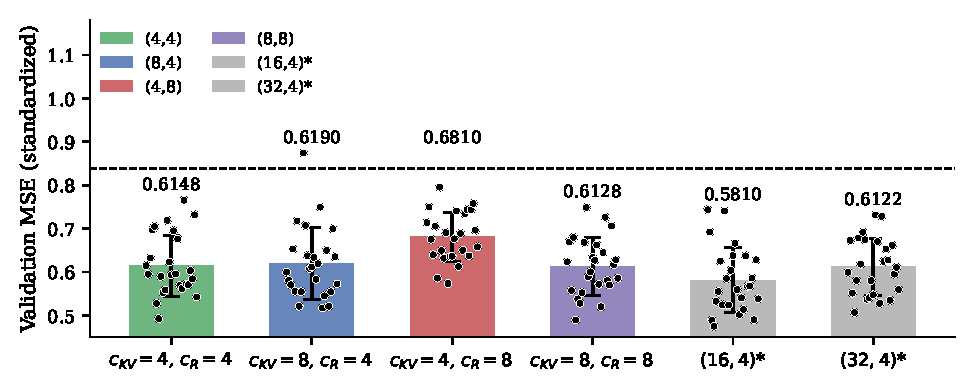
\includegraphics[width=0.92\linewidth]{figures/fig1_factorial_val.pdf}
\caption{Validation MSE by factorial cell (mean $\pm$ std over 5 paired
seeds; individual seed points shown). Lower is better. The champion corner
$(c_{KV}{=}8, c_R{=}4)$ combines coarse KV compression with fine routing.}
\label{fig:factorial}
\end{figure}

\textbf{Main effects.} Averaging over the opposite axis (Figure
\ref{fig:main-effects}): coarsening KV compression from $4{:}1$ to $8{:}1$
\emph{lowers} validation MSE by $-0.0427$ (mildly beneficial), while
coarsening routing resolution from $4{:}1$ to $8{:}1$ \emph{raises} it by
$+0.0463$ (deterioration). Both signs are consistent in 7 of 10
seed-column comparisons each.

\textbf{Pre-registered hypothesis H1} asked whether coarsening the router
deteriorates performance \emph{more} than coarsening KV compression. The
strict form is \emph{not} confirmed: the two effects are nearly equal in
magnitude ($0.0463$ vs.\ $0.0427$) and opposite in sign, so all observed
deterioration is attributable to routing while KV compression is mildly
beneficial. Both effect sizes (${\sim}0.04$) are smaller than the mean
within-cell seed standard deviation ($0.0647$; per-cell range
$0.0393$--$0.0875$), and no formal significance test was run. We therefore
report the decoupling direction as \emph{directional evidence}, not a
conclusive result (see the statistical treatment in
Section~\ref{sec:stats}; a mixed-effects model
$\mathrm{MSE} = \beta_0 + \beta_1 \log_2 c_{KV} + \beta_2 \log_2 c_R +
\beta_3 \log_2 c_{KV}\log_2 c_R + \text{random effects}$, with the main
claim requiring $\beta_2 > \beta_1$, is deferred until more cells and seeds
exist). Per-seed trajectories show the
ordering across cells is not unanimous for every seed---another reason the
champion claim is stated as ``best on mean,'' not ``best for every seed.''

\begin{figure}[t]
\centering
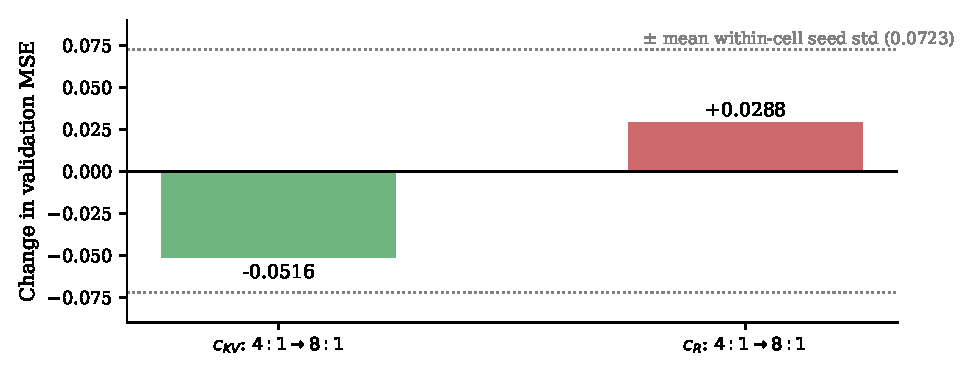
\includegraphics[width=0.92\linewidth]{figures/fig2_main_effects.pdf}
\caption{Main effects on validation MSE: $c_{KV}$ $4{:}1 \rightarrow 8{:}1$
($-0.0427$, mildly beneficial) and $c_R$ $4{:}1 \rightarrow 8{:}1$
($+0.0463$, deteriorates). Dashed lines: $\pm$ mean within-cell seed std
($0.0647$); both effects are smaller than seed noise.}
\label{fig:main-effects}
\end{figure}

\subsection{RQ2: compressed vs.\ full attention}
\label{sec:rq2}
Table~\ref{tab:baseline} compares full causal attention (Normal, 256
columns, no compression) with the two cells that anchor the family's
design corners, CSA $(4,4)$ and the champion DRRA $(8,4)$.
Every compressed cell beats Normal on mean validation
and mean test MSE, and \emph{every one of the 20 paired seed comparisons}
favors the compressed configuration (range of validation deltas
$-18.5\%$ to $-29.1\%$; the DRRA $(8,4)$ cell's advantage is the largest in 3 of
5 seeds, with CSA $(4,4)$ ahead at seeds 2024 and 99).

\begin{table}[t]
\centering
\small
\caption{Compressed vs.\ full attention (5 paired seeds, frozen protocol).
Deltas are computed on the 4-decimal means. Parameter counts are not
equalized across the three rows: Normal is a different attention class and
carries $\sim$2\% more full-model parameters.}
\label{tab:baseline}
\begin{tabular}{lccccc}
\toprule
Config & Val mean $\pm$ std & Test mean & $\Delta$val vs.\ Normal & $\Delta$test vs.\ Normal & Seeds beating Normal \\
\midrule
Normal & $0.8416 \pm 0.0799$ & 1.0814 & --- & --- & --- \\
CSA $(4,4)$ & $0.6332 \pm 0.0611$ & 0.9079 & $-24.76\%$ & $-16.04\%$ & 5 / 5 \\
DRRA $(8,4)$ & $\mathbf{0.5967} \pm 0.0710$ & $\mathbf{0.7988}$ & $-29.10\%$ & $-26.13\%$ & 5 / 5 \\
\bottomrule
\end{tabular}
\end{table}

\textbf{Wiring verification.} Because the compressed variants beating an
unmodified baseline by ${\sim}25$--$29\%$ is a surprising direction, we
audited the Normal attention implementation before reporting it: a
from-scratch naive reference (true causal masking, $1/\sqrt{d}$ scaling,
independent RoPE reimplementation) matches the module output
bit-exactly at $L{=}32$ and $L{=}64$ ($0.0$ max absolute difference) and to
$1.19 \times 10^{-7}$ at $L{=}256$ (fp32 accumulation noise); future
positions receive exactly zero weight and future-token perturbation leaves
outputs unchanged. The baseline is correctly implemented, so the comparison
stands. We also note the direction is surprising in the other sense:
compression acting as a task-appropriate inductive bias (see
Section~\ref{sec:discussion}) is a plausible but \emph{unverified}
explanation \emph{that three mechanistic probes now support descriptively}
(plan/gates/gate12/gate12\_summary.md): (i) on the delayed-copy dataset
(five channels periodic with in-window lags 96--256, plus two noise
channels), \emph{all three} models learn the exact-offset copy ---
per-channel copy MSE $0.0007$ (Normal) and $0.0013$--$0.0026$ (compressed
cells) against a noise floor of ${\approx}1.05$ --- so exact-offset recall
is not the differentiator, though Normal is ${\sim}2\times$ more precise
on the copy channels, with a mild lag gradient for the compressed cells;
(ii) on the change-point dataset, DRRA $(8,4)$ has the lowest per-window error
in \emph{every} distance-from-change bucket (the across-bucket gradient is
confounded by the generator's random-walk drift and should not be
over-read); and (iii) across the twelve datasets, the compression
advantage correlates with signal smoothness in the predicted direction
(Pearson $r = -0.29$ for DRRA $(8,4)$, $-0.35$ for CSA $(4,4)$ against lag-1
autocorrelation; $p \approx 0.3$) --- smoother series favor compression
more. These probes are descriptive ($n{=}1$ seed for (i)--(ii), $n{=}12$
for (iii)) and do not establish the mechanism.

\subsection{RQ3: cross-dataset coverage}
\label{sec:rq3}
To test whether the ETTh1 result is a single-dataset artifact, we repeated
the three-way comparison (Normal vs.\ CSA $(4,4)$ vs.\ DRRA $(8,4)$) on eleven
further datasets---three more ETT members, three large multivariate sets,
two different-dynamics sets, and three mechanistic synthetic families---under
the identical frozen protocol with the same five paired seeds (180 runs in
total; per-seed tables and the integrity audit in
plan/gates/gate3/gate3\_summary.md). Table~\ref{tab:coverage} and
Figure~\ref{fig:coverage} summarize validation MSE by dataset.

\textbf{Reading the table.} Table~\ref{tab:coverage} is transposed relative
to the earlier ones: each \emph{row} is a configuration (Normal, CSA $(4,4)$,
DRRA $(8,4)$, plus a $\Delta$val row for DRRA $(8,4)$ vs.\ Normal) and each
\emph{column} is one of the twelve datasets; a cell holds the mean
validation MSE over the five paired seeds, with the best mean per dataset
column in bold. Reading down a column compares the three models on one
dataset---e.g., ETTm2 is the suite's largest win for DRRA $(8,4)$ ($-48.4\%$),
while in the syn-delayedcopy column all three models agree within $0.001$
and Normal's mean is best. Reading across a row compares one model across
datasets, but \emph{columns are not comparable to each other}: every
dataset is standardized with its own train-only statistics, so MSE values
only have meaning within a column. The final $\Delta$val row is
scale-free (a ratio per dataset) and is therefore the row to compare across
columns; it also carries the honest exceptions---positive entries on
Exchange ($+8.6\%$) and on all three synthetic families ($+0.2\%$ to
$+3.1\%$).

The compressed configurations beat full attention on mean validation MSE in
8/12 datasets (DRRA $(8,4)$) and 7/12 (CSA $(4,4)$), but the advantage is
\emph{signal-dependent} rather than universal. The largest wins are on the
ETT family (up to $-48.4\%$ on ETTm2) and on solar-energy; both compressed
variants \emph{lose} on all three synthetic families ($+0.2\%$ to $+3.1\%$)
and on exchange-rate validation, and their test error is worse on weather
($+5.9\%$ and $+14.2\%$). This pattern is consistent with the
compression-as-inductive-bias reading: pooling adjacent timesteps is nearly
lossless on smooth, temporally redundant real-world series, while tasks
requiring exact in-window content recall (the delayed-copy probe,
known-period sinusoids) leave full attention with a slight edge. These
observations remain descriptive: five paired seeds per dataset, no
significance test, and the three rows are not parameter-equalized
($\sim$2\% full-model spread; the same stance as
Section~\ref{sec:rq2}).

\begin{table}[t]
\centering
\small
\caption{Cross-dataset validation MSE (5 paired seeds, frozen protocol;
pooled MSE in standardized units, lower is better). Models as rows,
datasets as columns; bold: best mean per dataset column. Column
abbreviations: Elec=Electricity, Traf=Traffic, Wea=Weather, Exc=Exchange,
Sol=Solar-Energy, sSin=syn-sinusoids, sCP=syn-changepts, sDC=syn-delayedcopy.
Full per-seed tables and integrity audit: plan/gates/gate3/gate3\_summary.md.}
\label{tab:coverage}
\setlength{\tabcolsep}{4pt}
\resizebox{\linewidth}{!}{%
\begin{tabular}{lrrrrrrrrrrrr}
\toprule
Model & ETTh1 & ETTh2 & ETTm1 & ETTm2 & Elec & Traf & Wea & Exc & Sol & sSin & sCP & sDC \\
\midrule
Normal    & 0.8416 & 1.9187 & 0.4285 & 1.5618 & 0.4047 & 0.5994 & 0.4460 & $\mathbf{2.9800}$ & 0.1899 & $\mathbf{0.1227}$ & $\mathbf{5.9456}$ & $\mathbf{0.2888}$ \\
CSA $(4,4)$   & 0.6332 & $\mathbf{1.3624}$ & 0.3965 & 0.9964 & $\mathbf{0.3798}$ & $\mathbf{0.5838}$ & 0.4469 & 3.1166 & $\mathbf{0.1721}$ & 0.1264 & 5.9677 & 0.2894 \\
DRRA $(8,4)$   & $\mathbf{0.5967}$ & 1.8080 & $\mathbf{0.3832}$ & $\mathbf{0.8053}$ & 0.3808 & 0.5874 & $\mathbf{0.4424}$ & 3.2350 & 0.1722 & 0.1264 & 6.0013 & 0.2894 \\
$\Delta$val DRRA $(8,4)$ vs Normal & $-29.1\%$ & $-5.8\%$ & $-10.6\%$ & $-48.4\%$ & $-5.9\%$ & $-2.0\%$ & $-0.8\%$ & $+8.6\%$ & $-9.3\%$ & $+3.1\%$ & $+0.9\%$ & $+0.2\%$ \\
\bottomrule
\end{tabular}}
\end{table}

\begin{figure}[t]
\centering
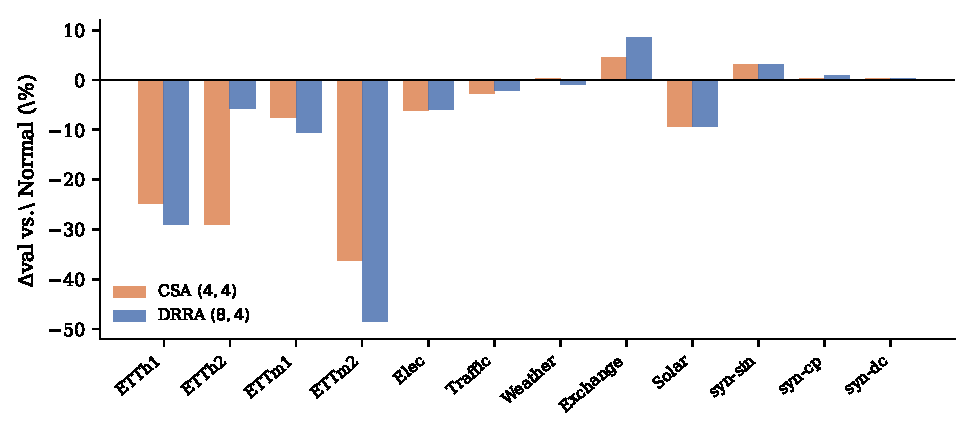
\includegraphics[width=0.92\linewidth]{figures/fig6_dataset_coverage.pdf}
\caption{Validation-MSE change vs.\ full attention by dataset (mean over 5
paired seeds): CSA $(4,4)$ (orange) and DRRA $(8,4)$ (blue). Compression helps on the
ETT family, solar, and electricity but slightly hurts on the synthetic
probes and exchange-rate validation.}
\label{fig:coverage}
\end{figure}

\subsection{Statistical treatment}
\label{sec:stats}
All comparisons above are descriptive. To make the evidentiary status
precise rather than implicit, we ran an analysis-only statistical pass on
the existing runs (no new training; log in plan/gates/gate4/gate4\_stats.md).
Per-dataset, the three comparisons (DRRA vs.\ Normal, CSA $(4,4)$ vs.\ Normal,
DRRA vs.\ CSA) were tested with exact paired Wilcoxon signed-rank tests
on validation MSE; \emph{nothing survives Holm correction across the 36
tests}, and with $n{=}5$ paired seeds the two-sided $p$-value floor is
$0.0625$, so no per-dataset effect \emph{can} reach $p < 0.05$ at this
sample size (the closest raw values are etth1 and solar at $0.0625$ in
favor of DRRA $(8,4)$; the synthetic probes are significant in the opposite
direction). Across datasets, paired sign tests on the 12 dataset means are
not significant either: DRRA $(8,4)$ beats Normal on mean validation MSE in 8/12
datasets ($p = 0.39$) and CSA $(4,4)$ in 7/12 ($p = 0.77$). The strongest
scale-free aggregate statement available is the bootstrap 95\% CI on the
mean of the per-dataset $\Delta$val vs.\ Normal: it excludes zero for both
variants (CSA $(4,4)$: $-8.9\%$ $[-16.8, -2.2]$; DRRA $(8,4)$: $-8.3\%$
$[-17.5, -0.8]$). We therefore state the results as directionally
consistent but not statistically established per dataset---the only
defensible claim at this sample size---and report these tests so that the
status is explicit rather than left to the reader. Deferred items, with
written justification in the project plan: the mixed-effects model
(Section~\ref{sec:rq1}), HAC/block-bootstrap corrections (the analysis is
at the seed level, where the five paired runs are independent, so stride-1
window overlap does not invalidate the paired tests), and TOST/ROPE (the
paper makes no equivalence claims).

\textbf{Sequence-length scaling and complexity.}
Figure~\ref{fig:lscale} sweeps the lookback $L \in \{128, \dots, 4096\}$ at
batch 1 and 32. At batch 32 the champion's advantage over Normal grows from
$-32\%$ at $L{=}512$ to $-56\%$ at $L{=}2048$ ($869$ vs.\ $1984$ ms/batch, a
$2.3\times$ speedup), and at batch 1/$L{=}4096$ it reaches $-63\%$ ($86$ vs.\
$235$ ms)---while at $L \le 256$ and batch 1 Normal is fastest (fixed overheads
again). The
empirical log-log slopes ($L \ge 512$) are $1.40$ (champion), $1.42$
(CSA $(4,4)$), and $1.72$ (Normal) at batch 32: consistent with the complexity
analysis of Section~\ref{sec:factorial}---the routing term
$O(L^2/c_R)$ keeps every cell asymptotically quadratic, with a reduced
constant for the compressed cells, and Normal approaches the quadratic
slope fastest. We therefore do \emph{not} claim subquadratic scaling. At
the extreme, batch-32/$L{=}4096$ full attention requires a ${\sim}8$ GB
score tensor and was skipped on the 16 GB machine---the practical memory
wall of dense attention that compressed attention avoids. All models
process the frozen task in under $2$ ms per sequence at batch 32 (mean
$1.6$--$1.8$ ms/seq at $L{=}256$; the $L{\ge}512$ region of the scaling
panel is where attention, not fixed overhead, dominates per-batch time).

\textbf{Compute and memory accounting.} Analytic forward MACs per sequence
(L=256, dominant terms; formulas in plan/gates/gate5/gate5\_bench.py):
Normal $76.9$M, CSA $(4,4)$ $61.7$M, DRRA $(8,4)$ $59.6$M --- the champion needs
$22\%$ fewer MACs than Normal. Two honest caveats: the wrapper MLP
($33.9$M) is the largest single block for \emph{every} model, so attention
is not the dominant compute at this scale; and measured latency differences
($-6\%$) are smaller than the MAC difference ($-22\%$) because dense-masked
CPU GEMMs are efficient relative to the extra compressor/indexer work.
Peak resident memory during a batch-32 forward burst grows by
${\sim}0.3$ GB (process watermark; parameter memory is only ${\sim}1.4$ MB
per model), and at batch-32/$L{=}4096$ the full-attention score tensor
(${\sim}8$ GB) exceeds the 16 GB machine. Training time over the fixed
10-epoch ETTh1 budget (parsed from the sweep log; medians of 5 runs):
Normal $474$ s, CSA $(4,4)$ $511$ s, DRRA $(8,4)$ $459$ s --- one DRRA run
($1417$ s) overlapped a machine-sleep window and is excluded from the
median. All latency/compute measurements are single-machine (Apple M2,
fp32, 8 threads); cross-hardware transfer (Linux x86, GPU) and model
depth/width sweeps remain future work (Appendix roadmap item~4).

\begin{figure}[t]
\centering
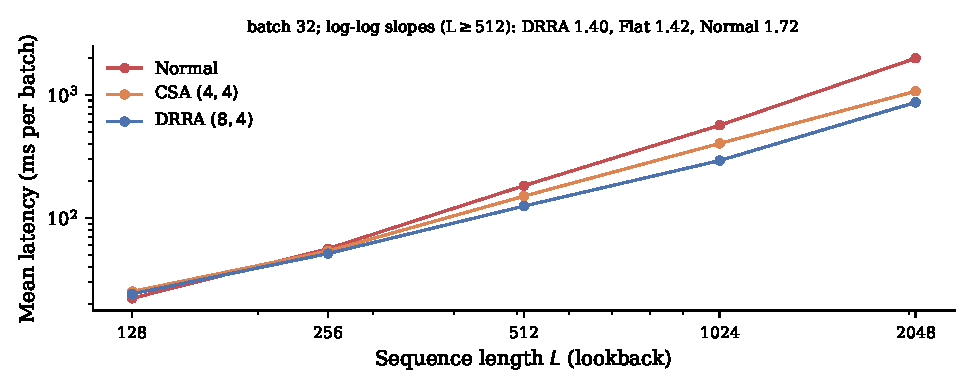
\includegraphics[width=0.92\linewidth]{figures/fig8_lscale.pdf}
\caption{Forward-pass latency vs.\ lookback length $L$ (log-log; batch 32;
mean over per-round medians). All cells are asymptotically quadratic
(routing term $O(L^2/c_R)$); the compressed cells have smaller constants
and lower empirical slopes ($1.40$/$1.42$ vs.\ $1.72$ for Normal at batch
32), and batch-32/$L{=}4096$ full attention exceeds practical memory (see
text). Measurement log: plan/gates/gate5/gate5\_bench.py +
gate5\_results.json.}
\label{fig:lscale}
\end{figure}

\subsection{Efficiency}
\label{sec:efficiency}
Table~\ref{tab:configs} gives the structural efficiency story: the
champion attends to 48 columns per query (5.3$\times$ fewer than Normal)
at 95{,}652 attention parameters---\emph{fewer} than Normal's 102{,}496---and
a full-model count 2.0\% below Normal's. Routing cost is identical for the
two $c_R{=}4$ cells regardless of $c_{KV}$, which is the deliberate
trade-off: pay the full fine-routing cost, halve the attention cost.

Table~\ref{tab:speed} reports wall-clock forward-pass latency measured
\emph{now} under the frozen protocol on the development machine, using the
alternating head-to-head protocol (all three models timed in rotation within
each round, so each round shares the same thermal/contention window; 25
rounds of 30 passes after warm-up; mean over per-round medians with 95\%
percentile bootstrap CIs, plus p90/p99 tails). The champion has the lowest
mean latency ($49.3$ ms vs.\ $52.5$ ms for Normal, $-6.1\%$; CSA $(4,4)$
$-0.7\%$), and the ordering $(8,4) < (4,4) <$ Normal replicated across a
second run, but the 95\% CIs overlap and the level shifts by
${\sim}6$--$9\%$ between runs (thermal and contention effects), so we report
the latency comparison as \emph{directional} only. Notably, the structural
5.3$\times$ column reduction does not translate into proportional wall-clock
gains at this scale: dense-masked CPU GEMMs are efficient and the
compressor/indexer add overhead. These are single-machine CPU measurements
(fp32, 8 threads); cross-hardware transfer (Linux x86, GPU) remains
follow-up work (Appendix roadmap item~4).
The pilot-era speed figures from earlier stages of this project remain
superseded and are not used here.

\textbf{Batch-size scaling.} Figure~\ref{fig:latency-scale} shows how the
comparison changes with the number of input windows processed per forward
pass (mean ms per sequence). At batch size 1 the fixed per-model overheads
(compressor, indexer) dominate and Normal is fastest ($2.5$ vs.\ $3.3$
ms/seq for DRRA $(8,4)$, $+30.8\%$). From batch 8 onward the compressed cells run
at or below Normal, and at large batches the attention-column reduction
takes over: the DRRA $(8,4)$ mean advantage over Normal is $-6.1\%$ at batch 64,
$-5.1\%$ at 100, $-10.5\%$ at 128, and $-21.1\%$ at 256 ($3.49$ vs.\ $4.42$
ms/seq). At the mid-range batches 16--32 the two are within run-to-run
noise (the scaling run shows $-0.1$ to $+0.2\%$ there while the canonical
Table~\ref{tab:speed} run shows $-6.1\%$ at batch 32). The overall pattern
is the expected signature of amortized overheads: the compression machinery
costs fixed work per pass, while the saved attention columns scale with the
batch.

\textbf{Synthesis: is the dual-rate design better?} Each table speaks to one
axis of ``better.'' Table~\ref{tab:configs} establishes the \emph{structural}
side: DRRA $(8,4)$ needs 48 attention columns (5.3$\times$ fewer than Normal),
slightly fewer parameters than Normal, and the same fine-routing candidate
count as the equal-rate cells. Tables~\ref{tab:factorial}--\ref{tab:coverage}
establish the \emph{accuracy} side: the champion beats Normal on mean
validation MSE in 8/12 datasets and has the best factorial cell on ETTh1,
with effects that are directional and, on the synthetic probes and some
datasets, reversed. Table~\ref{tab:speed} and Figure~\ref{fig:latency-scale}
establish the \emph{measured-latency} side: the champion has the lowest mean
latency at batch sizes $\ge 64$ (to $-21\%$ at 256) but is not statistically
separated from Normal at batch 32, and is slower at batch 1. Read together,
the evidence favors DRRA $(8,4)$ on every axis---geometry, parameters, accuracy
on most datasets, large-batch latency---but none of the advantages clears a
significance or noise threshold on its own, and the accuracy advantage is
dataset-dependent. We therefore state the conclusion as \emph{directional
superiority under this protocol on most datasets}, not a universal or
statistically established claim.

\textbf{Combined performance--speed view.}
Figure~\ref{fig:perf-speed} shows performance and speed \emph{together},
without collapsing them into a single score: the y-axis is the mean test
\emph{loss on ETTh1} (the frozen-task benchmark dataset, where all three
models share the same standardized scale; per-dataset losses across the
suite are \emph{not} averaged, because each dataset is standardized with
its own train-only statistics), and the x-axis is the mean forward-pass
\emph{latency} (lower latency = faster, i.e.\ the left side), at the frozen
batch 32 (left) and at batch 256 (right). Both axes are zoomed to the
measured range so the differences are visible; points are the five-seed
means, with no error bars shown. The best model in this view is the one in
the lower-left: \textbf{DRRA $(8,4)$} has the lowest mean test loss on ETTh1
($0.799$ vs.\ $0.908$ for CSA $(4,4)$ and $1.081$ for Normal) and the lowest
latency at both operating points ($49.3$ vs.\ $52.1$/$52.5$ ms at batch 32;
$892$ vs.\ $1171$/$1132$ ms at batch 256). CSA $(4,4)$ sits between the two on
both axes; Normal is upper-right (worst on both axes). Two honest readings:
at the frozen batch 32 the latency gap is a few milliseconds (within noise
at this scale), while at batch 256 DRRA $(8,4)$ is ${\sim}21\%$ faster; both
panels remain descriptive (five seeds per dataset, no significance tests,
single machine).

\begin{figure}[t]
\centering
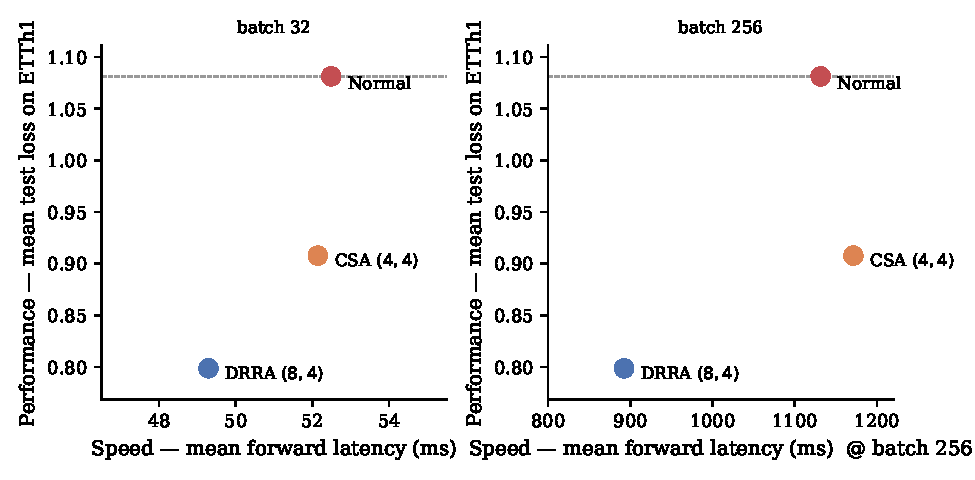
\includegraphics[width=0.92\linewidth]{figures/fig9_perf_speed.pdf}
\caption{Performance vs.\ speed: y-axis = mean test loss on ETTh1 (mean
over the five paired seeds; lower is better); x-axis = mean forward
latency (lower is faster, i.e.\ the left side); left: batch 32, right:
batch 256. DRRA $(8,4)$ is lower-left at both operating points --- the best
combined performance--speed choice --- with the separation growing at
batch 256. Measurement logs: plan/gates/gate3/gate3\_latency*.json +
gate3\_results/*.jsonl.}
\label{fig:perf-speed}
\end{figure}

\begin{figure}[t]
\centering
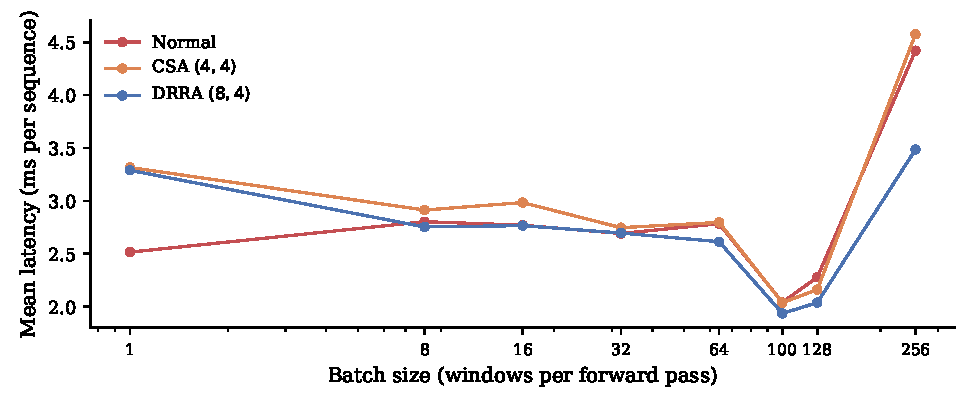
\includegraphics[width=0.92\linewidth]{figures/fig7_latency_scale.pdf}
\caption{Mean forward-pass latency per sequence vs.\ batch size under the
frozen protocol (development machine, fp32, 8 threads; mean over per-round
medians, 15 rounds $\times$ 15 passes per model per batch size). At batch
size 1 the fixed overheads of the compressor/indexer dominate and Normal is
fastest; from batch 64 onward DRRA $(8,4)$ is clearly fastest, with the gap
widening to $-21\%$ at batch 256. Measurement log:
plan/gates/gate3/gate3\_latency\_scale.py + gate3\_latency\_scale.json.}
\label{fig:latency-scale}
\end{figure}

\begin{table}[t]
\centering
\small
\caption{Forward-pass latency under the frozen protocol on the development
machine (Apple M2, 8 cores, 16 GB; CPU PyTorch 2.6.0, fp32, 8 threads).
Latency is the wall-clock time of \emph{one forward pass over a batch of 32
input windows} ($L{=}256$, $H{=}96$, $F{=}7$); per-sequence latency at this
batch size is mean$/32$ (${\approx}1.5$ ms/seq for DRRA $(8,4)$). Alternating
head-to-head protocol (25 rounds $\times$ 30 passes, warm-up excluded);
mean over per-round medians (95\% percentile bootstrap CI in brackets), with
p90/p99 tails; throughput from the mean pass time. Measurement log:
plan/gates/gate3/gate3\_latency.py + gate3\_latency.json.}
\label{tab:speed}
\begin{tabular}{lccccc}
\toprule
Model & Mean (ms) & p90 (ms) & p99 (ms) & $\Delta$mean vs.\ Normal & Throughput (batches/s) \\
\midrule
Normal & 52.5 $[50.4, 54.7]$ & 59.4 & 65.0 & --- & 19.1 \\
CSA $(4,4)$ & 52.1 $[49.2, 55.4]$ & 63.5 & 71.5 & $-0.7\%$ & 19.2 \\
DRRA $(8,4)$ & 49.3 $[47.2, 51.7]$ & 56.5 & 65.9 & $-6.1\%$ & 20.3 \\
\bottomrule
\end{tabular}
\end{table}

\section{Discussion}
\label{sec:discussion}

\subsection{The decoupling insight (directional)}
The cleanest reading of the factorial is that the two axes play different
roles on ETTh1: \emph{routing granularity carries accuracy; KV content density
is mildly beneficial to accuracy and buys efficiency}. The control logic is
internal to the design: the DRRA $(8,4)$ cell (coarse content, fine router) matches
or beats the equal-rate cells with roughly three-fifths the attention columns
(49 vs.\ 81 complete columns), while the $(4,8)$ cell (fine content, coarse
router) is the worst cell despite having the same columns as CSA $(4,4)$.
The per-seed consistency (19/25 in the same direction for each effect), the
pre-registered H1 contrast (exact Wilcoxon $p = 0.0023$), and the non-significant
interaction ($p = 0.31$) establish this as a \emph{statistically supported sign
structure on ETTh1}; the effect sizes remain modest relative to seed noise (both
effects ${\sim}0.03$--$0.05$ vs.\ within-cell std ${\sim}0.07$), the DRRA-vs.-CSA
edge itself is directional ($p = 0.096$), and multi-dataset confirmation of the
full factorial is still future work before this can be stated as a general design
principle.

\subsection{Why might compression help on this task?}
We do not have a verified explanation for the compressed $>$ full-attention
outcome, and we explicitly do not claim one. Candidate (unverified)
explanations include: compression acting as an inductive-bias regularizer;
the block structure effectively smoothing the attention field over
multi-step correlations; and the fixed 10-epoch budget interacting with
optimization landscape differences. The cross-dataset pattern
(Section~\ref{sec:rq3}) is broadly consistent with the regularization
reading---compression helps most where adjacent timesteps are most
redundant (ETT family, solar, electricity) and slightly hurts on tasks
requiring exact in-window recall (the synthetic probes)---but it remains
descriptive evidence, not a verified mechanism. The pre-registered
hypothesis program (H1 is defined in Section~\ref{sec:rq1}) is designed to
separate the candidates, and its current status is:
\textbf{H1} (coarsening the router deteriorates accuracy more than
coarsening KV compression) directionally supported in the factorial;
\textbf{H2} (the dual-rate corner matches or beats the equal-rate cells while
using fewer attention columns), whose latency leg is supported directionally by the
systems measurements and whose accuracy leg is directional (best-mean ETTh1 cell,
DRRA-vs.-CSA $p = 0.096$; 8/12 datasets);
\textbf{H3} (dense masked attention wins in small-work regimes but loses in
large-work regimes), whose crossover shape is observed on a single machine;
\textbf{H4} (the compression advantage depends on signal properties such as
smoothness and redundancy), consistent with the cross-dataset pattern; and
\textbf{H5} (a distilled surrogate can replace attention at inference
without an accuracy loss), which is out of scope for this paper---deferred
to a separate publication (Appendix~\ref{sec:appendix-surrogate}). The
mechanistic analyses that
would separate the explanations (routing recall, lag localisation) remain
future work.

\subsection{Limitations}
\label{sec:limitations}
\begin{itemize}
  \item \textbf{Dataset breadth, not universality.} The full factorial is
        single-dataset (ETTh1); the three-way comparison spans twelve
        datasets, where the compressed advantage is signal-dependent
        (Section~\ref{sec:rq3}): wins on the ETT family, solar, and
        electricity; small losses on the synthetic probes, exchange-rate
        validation, and weather test error. No cross-scale claim is made
        (CPU-scale models only), and horizons beyond $H{=}96$ with lookbacks
        beyond $L{=}256$ are not yet evaluated.
  \item \textbf{Descriptive statistics.} Five paired seeds; per-dataset
        paired tests cannot reach significance at this sample size
        (two-sided floor $p = 0.0625$) and nothing survives Holm correction
        (Section~\ref{sec:stats}); ``best on mean'' and ``directional'' are
        used advisedly. No equivalence tests are run because no equivalence
        claims are made.
  \item \textbf{External architectures as reference points only.} DLinear
        and PatchTST were run under the frozen protocol to calibrate absolute
        error levels (Section~\ref{sec:refpoints}); they are not peer methods
        (different architectures, and DLinear has no attention), so no
        competitiveness claim is made. Efficiency-oriented peers (Informer's
        ProbSparse, iTransformer, TimesNet, SSM baselines) remain pending
        (Appendix future-work item~3).
  \item \textbf{Single-machine systems measurements.} Forward latency
        (batch and lookback scaling), MACs, memory, and training time are
        measured on the development machine (Table~\ref{tab:speed},
        Figure~\ref{fig:latency-scale} and~\ref{fig:lscale}). Cross-hardware
        results (Linux x86, GPU) and depth/width ablations are conscious
        scope exclusions, deferred to future work.
  \item \textbf{Non-IID samples.} Stride-1 windows overlap heavily; samples
        are not independent, which standard per-window significance tests
        would assume. Our paired tests are at the seed level (five
        independent runs), where the overlap does not invalidate them;
        block-bootstrap or HAC-robust corrections are deferred until
        per-window statistics are used (Section~\ref{sec:stats}).
  \item \textbf{Fixed budget, single checkpoint policy.} 10 epochs,
        epoch-10 weights; no early stopping or best-validation selection.
  \item \textbf{Single-block backbone retained.} The study keeps the minimal
        one-block backbone deliberately (the backbone, not the attention module,
        is the accuracy bottleneck at this scale, Section~\ref{sec:refpoints});
        forecast cost is reported both ways (full-layer and forecast-required,
        Section~\ref{sec:efficiency}), and a multilayer backbone remains future work.
  \item \textbf{CPU-only, fp32, small models.} Dense-with-masking
        implementation choices are CPU-oriented and may not transfer to
        GPU-flash-attention regimes.
\end{itemize}

\subsection{What this paper does not claim}
Consistent with the project's pre-registered warnings: this is not a novel
sparse-attention mechanism; it is not a state-of-the-art forecasting
system; the word ``equivalence'' is not used for any accuracy comparison;
no subquadratic claim is made beyond the structural column counts above;
and no component is claimed to be original. The contribution is the
controlled study, its measurements, and its honest boundaries.

\section{Conclusion}
\label{sec:conclusion}

We presented a controlled $2\times2$ factorial design study of
compressed-and-indexed attention for long-horizon time-series forecasting,
varying the KV compression rate $c_{KV}$ and the routing resolution $c_R$
independently under a frozen task, an auxiliary-identical contract, and
parameter equalization, across five paired seeds. On ETTh1 direct-96
forecasting, all compressed configurations outperformed full causal
attention ($-18.5\%$ to $-29.1\%$ validation MSE; 20/20 paired seed
comparisons; wiring-audited baseline), and the factorial separates the two
axes directionally: coarser routing deteriorates accuracy while coarser KV
compression is mildly beneficial, with the champion cell $(8,4)$ cutting
the attention matrix 5.3$\times$ at equal parameters. We deliberately stop
short of significance, generalization, or latency claims. The immediate
roadmap is statistical testing with temporal-dependence-aware methods,
multi-dataset replication, external baselines, and hardware latency
benchmarking; each is itemized in the appendix roadmap
(Appendix~\ref{sec:appendix-roadmap}).


\bibliographystyle{plainnat}
\bibliography{references}

\newpage
\appendix
\section{Documented negative results}
\label{sec:appendix-negatives}
Six failed designs were tried and documented during the development of this
family (each with runnable or archived implementations and failure modes):
sparse-gather routing ($\sim$5$\times$ slower than dense masking on CPU);
a hierarchical (multi-scale pyramid) indexer (consistently worse than the
flat indexer); a multi-scale KV pyramid at 224 KV tokens
(overparameterized for the budget); a learnable block-bias offset (NaN
instability in $\sim$50\% of runs; root cause later traced to uninitialized
memory---`torch.empty' biases---and fixed); a linear-pool indexer with
gated residual KV (loses the per-head $\times$ per-dimension routing
flexibility of the softmax-overlap gate); and stacked $2{:}1 \rightarrow
2{:}1$ compression (harder to optimize within the budget). Negative results
of this kind are a deliberate part of the reproducibility package; they are
secondary to the paper's core claim.

\section{Surrogate attention (separate line of work)}
\label{sec:appendix-surrogate}
Distilling the attention block into a cheap inference-time student is a separate
line of work, deferred to a separate publication: it is \emph{not} part of this
paper's claims, and none of its numbers are apples-to-apples with the frozen-task
results in Section~\ref{sec:experiments} (they predate the frozen protocol). This
pointer exists only to acknowledge the overlap with attention-distillation work
\citep{goldstein2025radlads} and to record the retention decision: the surrogate
line, including the equal-budget small-transformer control and
distillation-epoch alignment, lives outside this manuscript.

\section{Reproducibility}
\label{sec:appendix-repro}
Every number in this paper traces to a repository artifact: the frozen task
specification (the sole authority on task definition), the pre-registered
factorial design, the run harness and its machine-readable results manifests
(125 factorial/baseline runs at $n{=}25$ + 180 cross-dataset runs + external
reference-point runs, JSONL), a verified
per-module parameter registry, causality-verification and wiring-audit
suites (all variants pass future-invariance and exact-zero-future-gradient
checks; the Normal baseline is bit-identical to a naive causal reference),
and a sanity-test suite covering shapes, gradients, parameter counts, and
tiny-task fitting (including a per-cell index-to-block mapping regression test).
Supplementary audits ship as machine-readable logs alongside the manifests: last-query
equivalence, the router gradient audit, canonical last-query latency with paired
deltas, the index-to-block mapping audit (with the pre-fix misrouting finding and
the re-run of the affected cells), and the unrounded 25-seed factorial
recomputation. Reported means and deltas are computed from the audited
manifests; the figure-generation scripts in this paper's source tree read
the same manifests, so every figure is regenerable. The freeze-clean
package --- environment lockfile, dataset SHA-256 manifests, automated
figure/table regeneration scripts, and runnable test suites (causality,
gradient masks, wiring audit, data integrity) --- is all in the repository.
The source tree is under git with a freeze baseline (commit recorded in
the project changelog); the remaining reproducibility steps
at release time are a tagged archive with a DOI (e.g., Zenodo) and the
official venue style swap.

\section{Future work}
\label{sec:appendix-roadmap}
Scope completed in this study versus open follow-ups, by axis:
\begin{enumerate}
  \item \textbf{Statistics.} Factorial-level inference is complete:
        $n{=}25$ paired seeds; paired Wilcoxon with
        Holm correction over cell-vs-Normal contrasts
        (Section~\ref{sec:stats}); per-seed main-effect contrast for H1.
        Deferred with justification: mixed-effects model (the $2\times2$ already
        identifies the three fixed effects; deferred as a robustness re-expression),
        HAC/block bootstrap (seed-level analyses), TOST/ROPE (no
        equivalence claims); temporal-dependence-aware statistics for the
        cross-dataset suite remain future work.
  \item \textbf{Datasets.} The suite covers
        the ETT family (ETTh1, ETTh2, ETTm1, ETTm2), large multivariate
        (Electricity, Traffic, Weather), different dynamics (Exchange,
        Solar-Energy), and three mechanistic synthetic families (sinusoids,
        change points, delayed-copy), all under the frozen protocol with 5
        paired seeds (180 runs; per-seed tables in the released results
        manifests). Remaining: horizon ($H \in \{192, 336, 720\}$)
        and lookback ($L \in \{512, 720, 1024\}$) sweeps.
  \item \textbf{Baselines.} DLinear \citep{zeng2023dlinear} and PatchTST \citep{nie2023patchtst}
        under the identical frozen protocol as external reference points,
        not peer methods (Section~\ref{sec:refpoints}): DLinear on all
        twelve datasets; PatchTST on the eight datasets where its
        channel-independent training fits the single-machine CPU budget
        (declared omissions on solar/electricity/traffic/weather).
        Remaining as future work: iTransformer, Informer, TimesNet, and an
        SSM baseline.
  \item \textbf{Hardware/latency.} Development-machine measurement is complete:
        Mean/p90/p99 forward latency with bootstrap
        CIs, throughput, analytic MACs, peak-memory accounting, training
        time, and batch/lookback scaling sweeps (batch 1--256,
        $L \in \{128, \dots, 4096\}$); see Section~\ref{sec:efficiency}.
        Remaining as future work: cross-hardware transfer (x86 CPU, GPU)
        and depth/width ablations --- conscious scope exclusions of this
        study.
  \item \textbf{Literature re-audit:} the 2026-08-16 sweep of the
        2024--2026 routing/compression-attention literature found no
        counterexample to the \emph{to our knowledge} claim
        (Section~\ref{sec:related}); a fresh sweep before locking the
        title remains good practice.
\end{enumerate}


\end{document}
